\section{Results}

\subsection{Datastructuring and storage}
Methods to connect R/qtl to XGAP/molgenisDB were writen in the R programming language using the molgenis R-API. 
To use the molgenis API for R an R-package named Rcurl \cite{Rcurl08} is used to make HTTP connections to the 
molgenis server.

\begin{figure}[ht]  
\centering
  \hfill
  \fbox{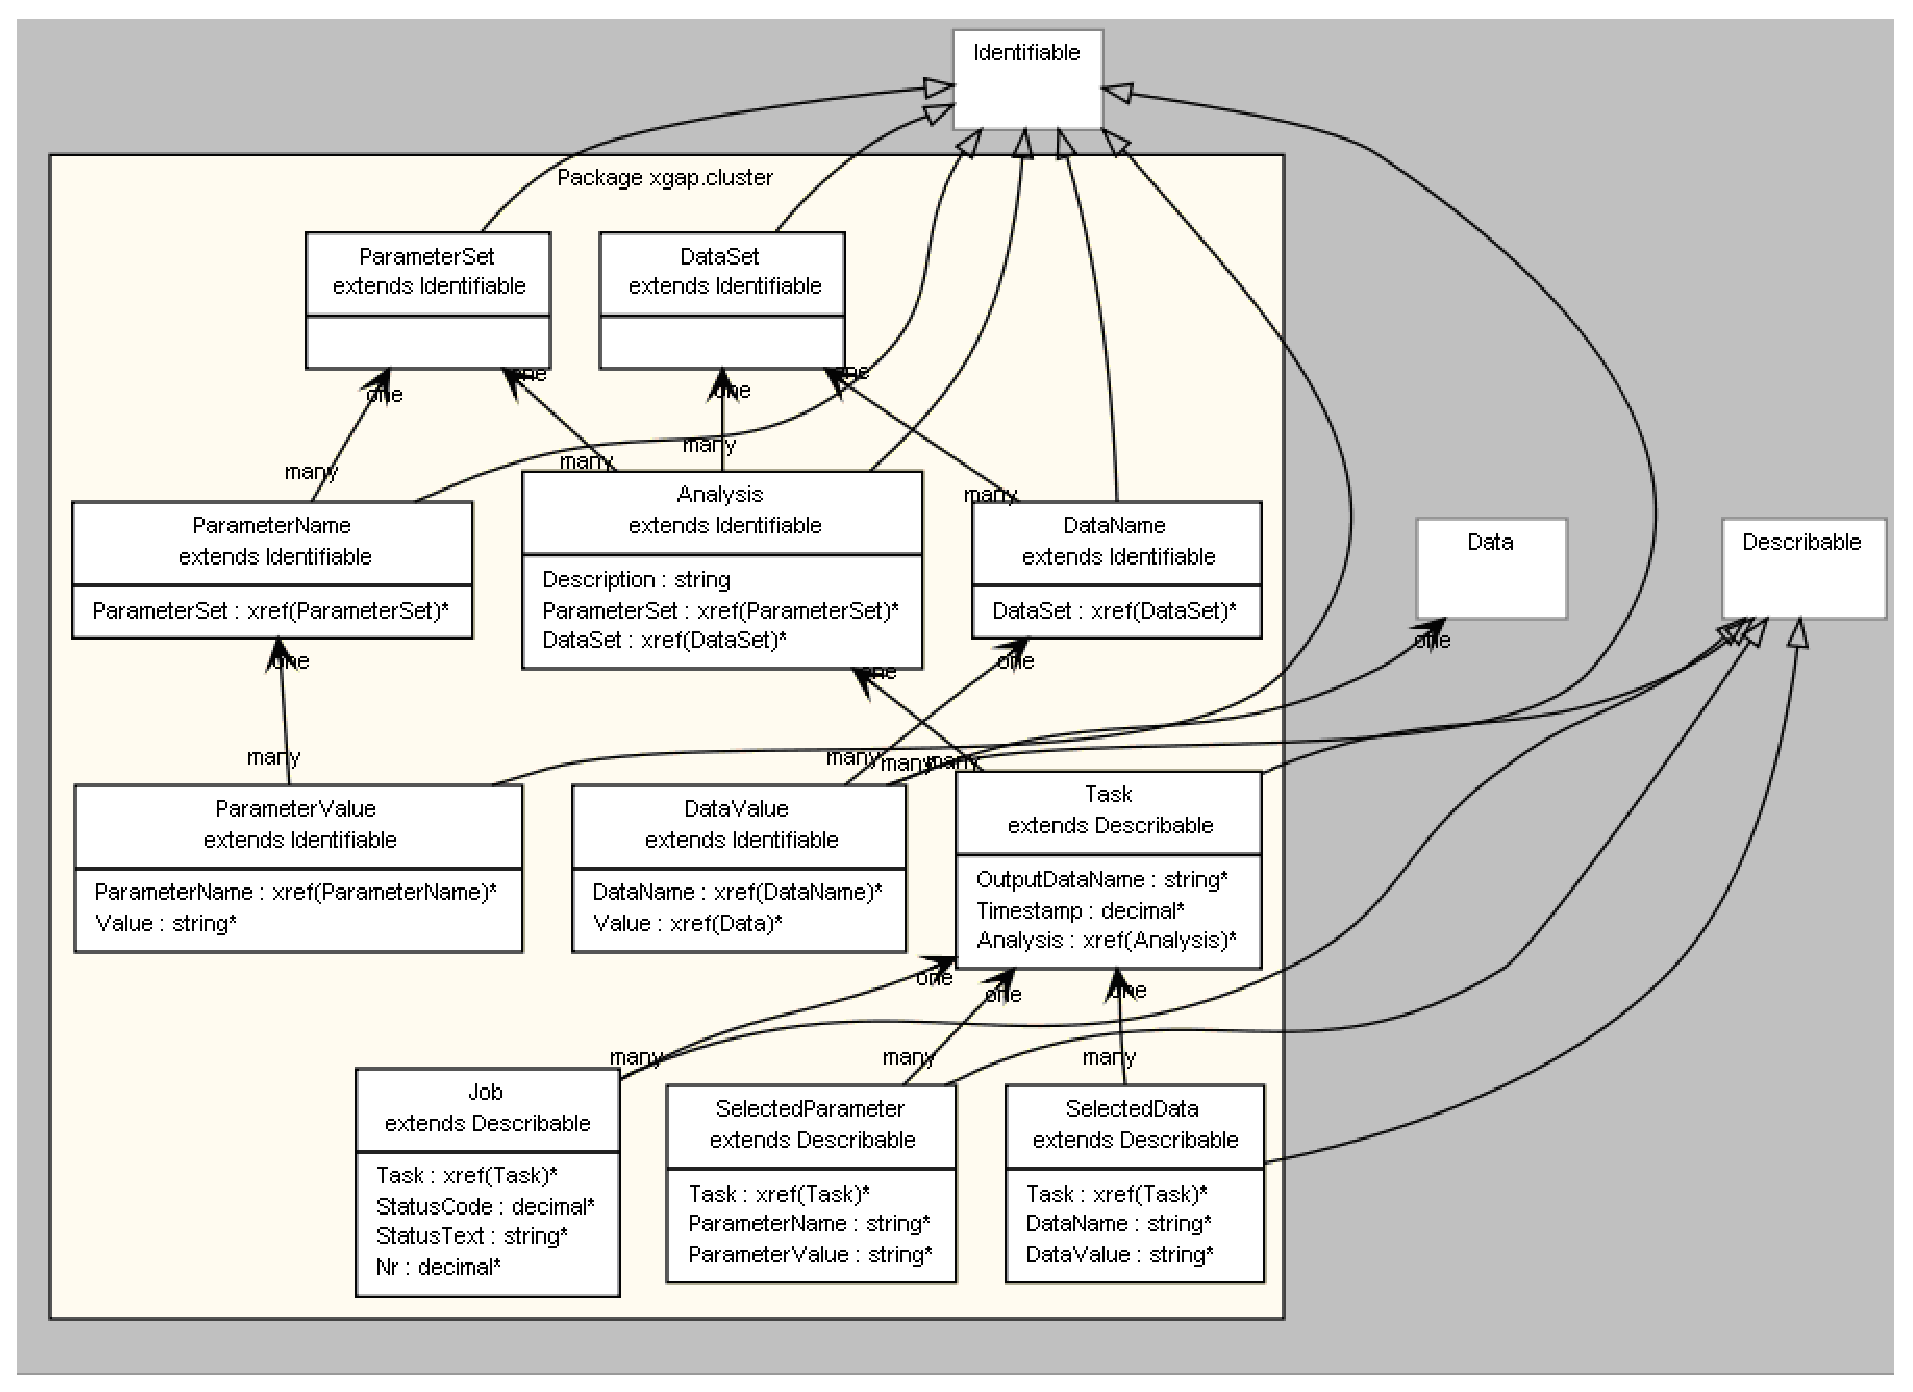
\includegraphics[height=8.0cm,width=15.0cm]{images/datamodel.eps}}
  \caption{Datamodel}
  \label{fig:FigDATAMODEL}    
\end{figure}

\begin{figure}[ht]  
\centering
  \hfill
  \fbox{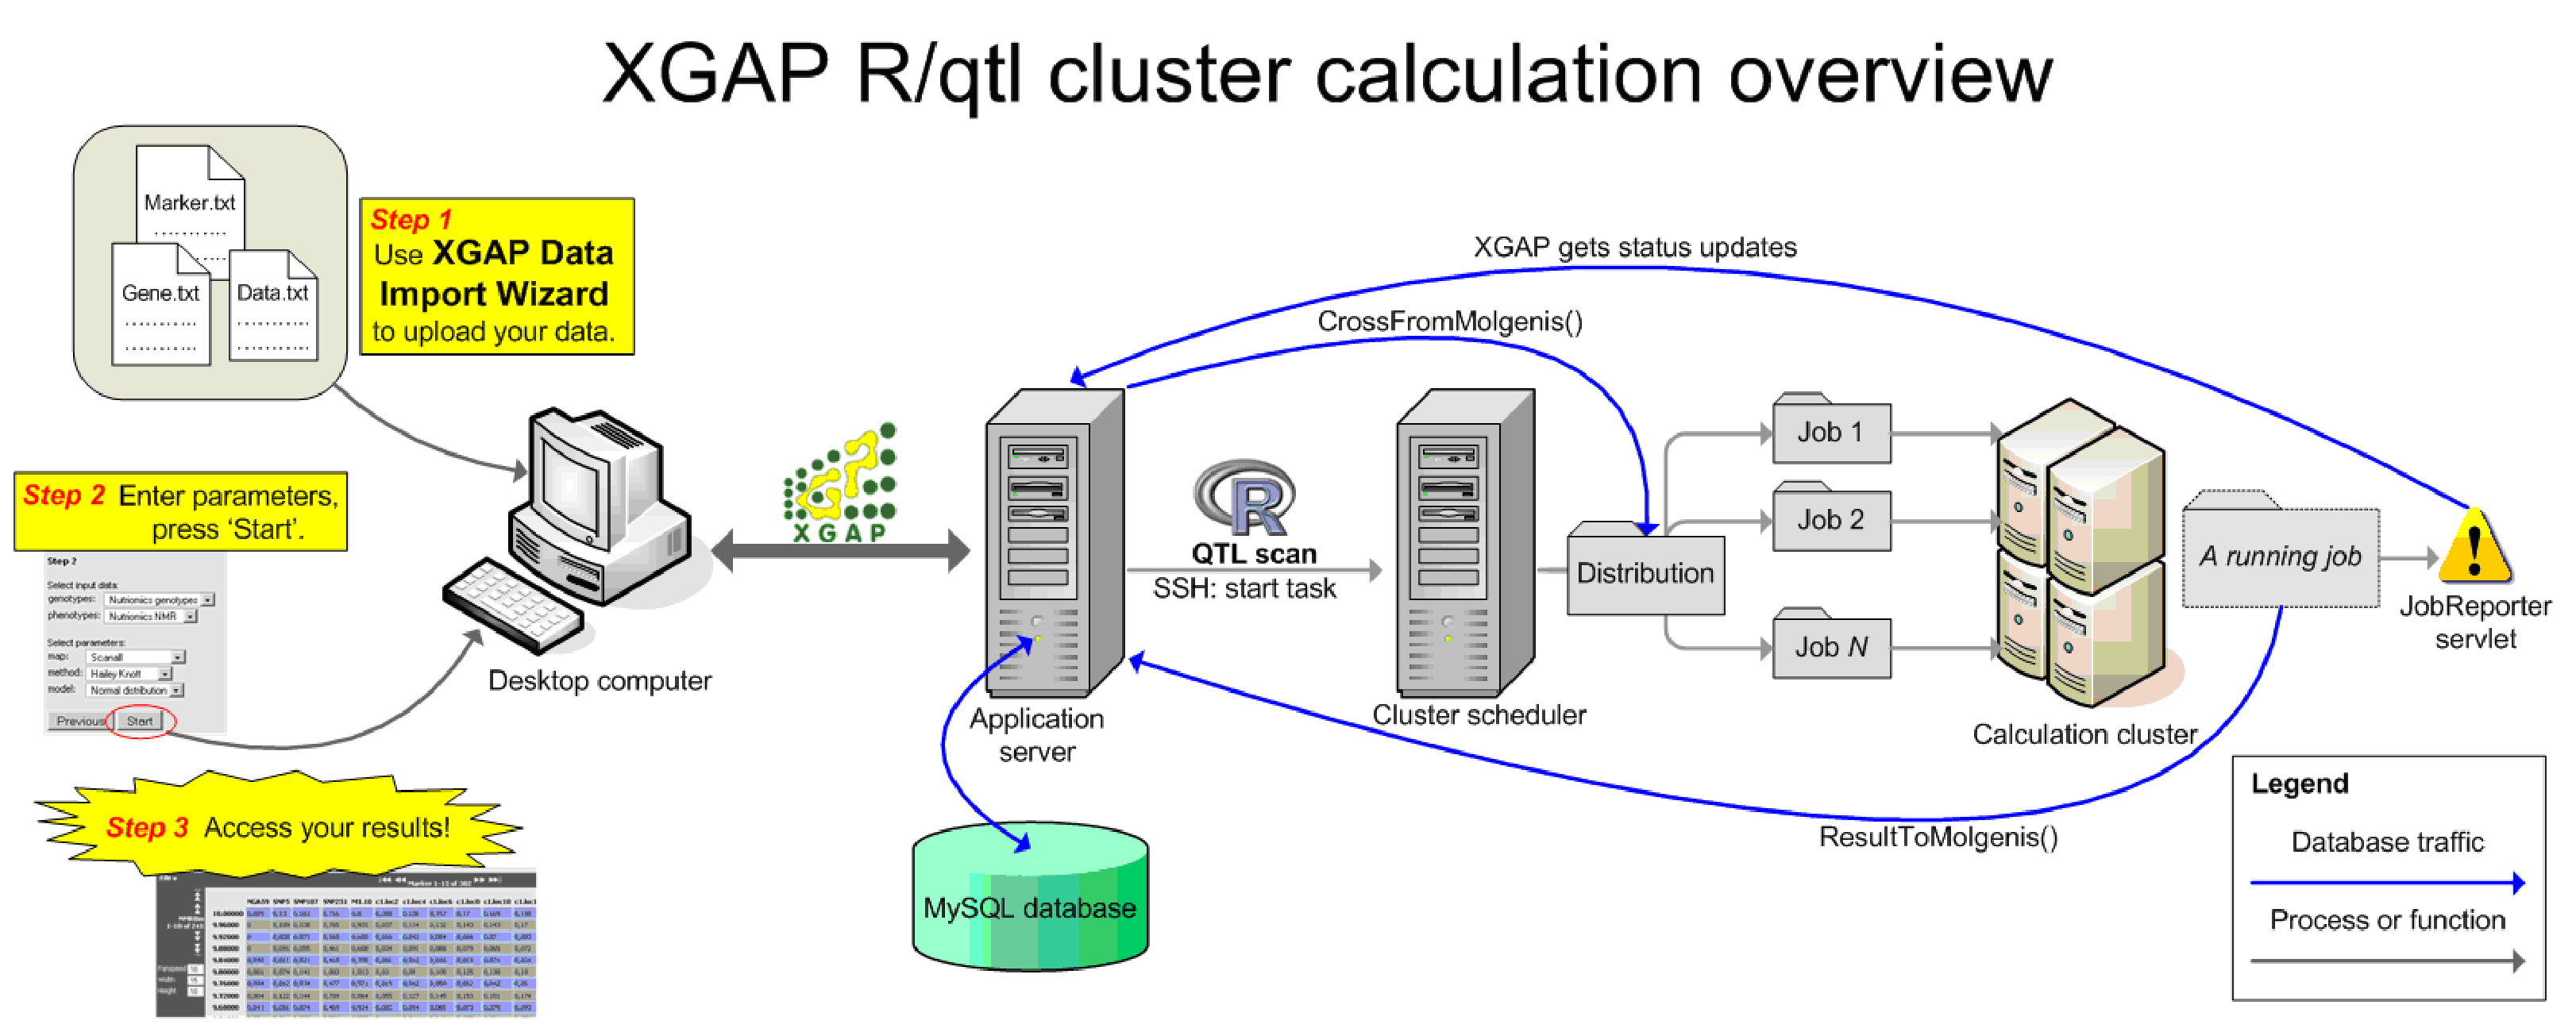
\includegraphics[height=8.0cm,width=15.0cm]{images/layout.eps}}
  \caption{Layout}
  \label{fig:FigLAYOUT}    
\end{figure}

\subsection{HPC of QTLs using molgenis}
Because there is a high threshold for biological users to use R for QTL analysis a webplugin into the molgenis system was created to enable users to 
use the molgenis webinterface to do highspeed parallelized QTL analysis. The plugin stores QTL profiles back into the database and also information about each run.
A webinterface provides users with a one click sollution, while the more complicated task are hidden out of sight. 
An overview of what happens out of sight can be seen in FIG XX.
The following functions are used during cluster analysis
\begin{itemize}
	\item CrossFromMolgenis() - Retrieving a dataset in the R/qtl cross format from a molgenis database system with the XGAP dataformat
	\item ResultsToMolgenis() - Storing results to a molgenis database system with the XGAP dataformat
	\item ResultsFromMolgenis() - Retrieving previously stored QTL analysis results from a molgenis database system with the XGAP dataformat
\end{itemize}

\begin{table}[ht]
	\caption{R/QTL parameters}
	\centering
	\begin{tabular}{| l | c | }
	\hline
	Scanall	&Main scanning interface of R/QTL created by K. Brohman et al\\
			&implementing per marker QTL analysis using different models and mapping methods.\\
	\hline
	MQMall	&Multiple QTL Mapping algorithm created by R.C. Janssen\\
			&implementing multiple QTL modeling and mapping using normal distributions.\\
	\hline
	CIMall	&Composite interval mapping created by G. Churchill and Senuk Sen\\
	\hline
	\end{tabular}
	\label{tbl:tabel0}
\end{table}

\begin{table}[ht]
	\caption{Reporter statuscodes}
	\centering
	\begin{tabular}{| l | c | c | }
	\hline
	-1	&Red	&An error has occurred.\\
	\hline
	0	&Orange	&Submitted to cluster as a potential job.\\
	\hline
	1	&Yellow	&Job is accepted and queued.\\
	\hline
	2	&Blue	&Job calculation done and is now uploading results back to the database.\\
	\hline
	3	&Green	&Job is completed.\\
	\hline
	\end{tabular}
	\label{tbl:tabel1}
\end{table}

